\documentclass[article]{jss}

%% -- LaTeX packages and custom commands ---------------------------------------

%% recommended packages
\usepackage{thumbpdf,lmodern}

%% another package
\usepackage{framed}
\usepackage{amsmath,amsthm}
\usepackage{amsfonts}
\usepackage{amssymb}
\usepackage{rotating}
\usepackage{orcidlink}
\usepackage{enumerate}
\usepackage{float} % to allow H for figure position
\usepackage{longtable}
\usepackage[tableposition=below]{caption}
\captionsetup[longtable]{skip=0.9em}
\usepackage{subcaption}
\usepackage{cleveref}
\usepackage{todonotes}
\usepackage{enumitem}
\usepackage{comment}


%arxiv
\usepackage{lmodern}

% track changes
\usepackage[]{changes}

%Algorithm
\usepackage{algorithm}
\usepackage{algorithmic}

%% new custom commands
\newcommand{\class}[1]{`\code{#1}'}
\newcommand{\fct}[1]{\code{#1()}}
\theoremstyle{definition}
\newtheorem{definition}{Definition}

\input{notation.tex}


%% -- Article metainformation (author, title, ...) -----------------------------

%% - \author{} with primary affiliation
%% - \Plainauthor{} without affiliations
%% - Separate authors by \And or \AND (in \author) or by comma (in \Plainauthor).
%% - \AND starts a new line, \And does not.
%\author{Sebastian Fischer \And Lukas Burk \And Florian Pfisterer \And Carson Zhang \AND Bernd Bischl \And Martin Binder}
\author{Sebastian Fischer~\orcidlink{0000-0002-9609-3197} \\
    LMU Munich \\
    MCML \\
    \And Lukas Burk~\orcidlink{0000-0001-7528-3795} \\
    LMU Munich \\
    MCML\\
    BIPS \\
    University of Bremen
    \And Florian Pfisterer~\orcidlink{0000-0001-8867-762X} \\
    \AND Carson Zhang \\
    LMU Munich \\
    \And Bernd Bischl~\orcidlink{0000-0001-6002-6980} \\
    LMU Munich \\
    MCML \\
    \And Martin Binder~\orcidlink{0009-0008-2578-2869} \\
    LMU Munich \\
    MCML \\
}

\Plainauthor{Sebastian Fischer, Lukas Burk, Florian Pfisterer, Carson Zhang, Bernd Bischl, Martin Binder}

%% - \title{} in title case
%% - \Plaintitle{} without LaTeX markup (if any)
%% - \Shorttitle{} with LaTeX markup (if any), used as running title
\title{mlr3torch: A Deep Learning Framework in R based on mlr3 and torch}
\Plaintitle{mlr3torch: A Deep Learning Framework in R based on mlr3 and torch}
\Shorttitle{\pkg{mlr3torch}: A Deep Learning Framework in \proglang{R} based on \pkg{mlr3} and \pkg{torch}}


%% - \Abstract{} almost as usual
\Abstract{
    Deep learning has become a fundamental approach in modern machine learning with applications across various domains.
    We introduce the \proglang{R} package \pkg{mlr3torch}, a comprehensive and extensible deep learning framework that integrates seamlessly into the \pkg{mlr3} machine learning ecosystem.
    Built upon the \pkg{torch} package, it simplifies the creation, training and evaluation of neural networks for both tabular data and generic tensors such as images.
    The package offers multiple levels of customization: predefined architectures, graph-based network construction, and full compatibility with \pkg{torch}.
    The representation of neural networks as graphs is built upon the graph-language defined in the \pkg{mlr3pipelines} \proglang{R} package and allows to define the whole deep learning workflow, including preprocessing, data augmentation and network architecture, in a single graph.
    By being fully integrated into the \pkg{mlr3} ecosystem, the package allows for standardized resampling, benchmarking, preprocessing, hyperparameter tuning and more.
    We explain the basic functionality of the package and how it can be customized or extended to new domains.
    We showcase the package's capabilities through applications such as neural architecture search, fine-tuning pretrained models, and defining architectures for multi-modal data, along with runtime benchmarks.
}

%% - \Keywords{} with LaTeX markup, at least one required
%% - \Plainkeywords{} without LaTeX markup (if necessary)
%% - Should be comma-separated and in sentence case.
\Keywords{deep learning, machine learning, \rlang{}}
\Plainkeywords{deep learning, machine learning, R}

%% - \Address{} of at least one author
%% - May contain multiple affiliations for each author
%%   (in extra lines, separated by \emph{and\$.
%% - May contain multiple authors for the same affiliation
%%   (in the same first line, separated by comma).
\Address{
  Sebastian Fischer \\
  Insitut f\"ur Statistik \\ Ludwig-Maximilians-Universit\"at M\"unchen, Germany \\
  Ludwigstr. 33, 80539 Munich, Germany \\
  Munich Center for Machine Learning (MCML), Germany \\
  E-mail: \email{sebastian.fischer@stat.uni-muenchen.de}
}

% https://www.jstatsoft.org/mission#types-of-papers
% Full reproducibility is mandatory for publication and the source code is published along with the article.
%  A careful comparison with other open-source implementations of similar models or procedures should highlight the capabilities of all implementations and the corresponding advantages or disadvantages.
% A description of the design principles and the actual implementation is at the heart of an JSS article.

% All new submissions must provide the following attachments:

%    PDF manuscript in JSS style,
%    source code for the software and
%    replication materials for all results from the manuscript, preferably via a single, commented standalone replication script.


% Software Preparation:
% Source code must be submitted in ASCII files.
% For R packages, we encourage inclusion of JSS submissions as vignettes in the package.
% Maximum Upload Size: 50 MB

% Style guide: https://www.jstatsoft.org/style

% Paper should not be longer than 30 pages

\begin{document}

\begin{comment}

Fullfilled:

\begin{itemize}
    \item Code distributed with JSS articles uses the GNU General Public License (GPL) version 2 or version 3 or a GPL-compatible license. JSS does NOT consider software distributed under other licenses.
\end{itemize}

Final submission:

\begin{itemize}
    \item [ ] Size limit: Upload not more than 50 MB
    \item [ ] submission must contain: pdf manuscript, source code, replication materials
    \item [ ] the manuscript must be fully and exactly reproducible on at least one platform
    \item [ ] We need to provide a simplified version of the script reproducing the results that can run on a regular PC. (https://www.jstatsoft.org/authors#manuscript-preparation) -> maybe I can just run this on GitHub actions CI?
    \item [ ] to facilitate review, authors are strongly encouraged to provide an output file that shows the results from running the single standalone replication script so that this can be compared against the results presented in the manuscript. For R submissions, this should be done by providing a file "code.html" created by running knitr::spin("code.R") on the replication script "code.R" which should include a call to sessionInfo() at the end.
    \item [ ] Source code must be submitted in ASCII files (but need to read software preparation guidelines again after submission: https://www.jstatsoft.org/authors#manuscript-preparation)
    \item [ ] manuscript can be compiled using pdflatex
    \item [ ] Special naming for programming languages and journals (don't think it applies here)
\end{itemize}

JSS Guides:

\begin{itemize}
    \item Should read https://stats-devguide.ropensci.org/ (more as general guidance, not a requirement for packages reviewed by JSS)
    \item !!!discuss the advantages and disadvantages of the new contribution compared to existing implementations, when possible and also applicable using empirical illustrations.
    \item Page limit: not longer than 30 pages
\end{itemize}

JSS Style guide:

\begin{itemize}
    \item [ ] Abbreviations should be spelled in upper-case letters without additional formatting (i.e., without periods, without small caps, italics, etc.). All abbreviations should be introduced with their expansion where the expansion should not be capitalized. (Exceptions are, of course, when the expansion contains proper names or the first word is the first word of a sentence.) Examples would include:
    \item [ ] never use (\cite{...}). (use \citep{} for that)
    \item [ ] \proglang, \pkg and \code have been used for highlighting throughout the paper (including titles and references), except where explicitly escaped.
    \item [ ] In order to use markup in section headers, you can use: \section[Calling C++ from R]{Calling \proglang{C++} from \proglang{R}}
    \item [ ] \title in title style
    \item [ ] \section, \subsection, etc. in sentence style (in sentence style, only first word of sentence and forst word after - or : is capitalized)
    \item [ ] annotations of figures/tables (including captions) in sentence style
    \item [ ] Figures, tables and equations are marked with a \label and referred to by \ref, e.g., Figure~\ref{...}
    Software packes are \cite{}d properly.
    \item [ ] Use \code{...} instead of \texttt{...} for inline code
    \item [ ] No comments in Code, this information should be presented in the normal latex text
    \item [ ] In all cases, code input/output must fit within the normal textwidth of the manuscript.
    \item [ ] Text in figures: In particular, this means that annotations should not be too large or too small. As a rough guidance, graphics annotation should be a about the size of the figure caption or a little bit smaller.
    \item [ ] For books with an edition, this should be indicated as 2nd, 3rd, etc.
    \item [ ] For referring to subsections, do not use Subsection x.y, just Section x.y.
    \item [ ] Add comma after e.g., and i.e., to prevent latex from interpreting as end of sentence
    \item [ ] use \top instead of ^T
    \item [ ] To refer to equations, one can use either Equation~\ref{...} (with capitalization) or (\ref{...}) with the former being preferred if the number of equation references is not too large.
\end{itemize}

References:

\begin{itemize}
    \item all titles in the BibTeX file in title style.
    \item Use \proglang{} and \pkg{} also there
    \item If software does not say provide way for citation, use  the following:
    \@Manual{SAS-STAT,
        author  = {{\proglang{SAS} Institute Inc.}},
        title   = {\proglang{SAS/STAT} Software, Version~9.1},
        year    = {2003},
        address = {Cary, NC},
        url     = {https://www.sas.com/}
    }
    \item For R packages that don't have an official citation, use citation("foo"), but make sure that \proglang{} and \pkg{} are used correctly
\end{itemize}


Captions:

\begin{itemize}
    \item All captions should appear below the corresponding figure/table.
    \item The captions should be in sentence style and end with a period. No additional formatting (such as \emph, \bf or \it) should be used for the caption.
    \item All table row/column headers should also be in sentence style. There should not be further footnote-style annotations in tables; these should all be placed in the caption.
\end{itemize}

Susanne's review:

\begin{itemize}
    \item For bullet lists/itemized lists please use either a comma, semi-colon, or period at the end of
each item
    \item Do not use additional formatting for specific words unless explicitly required by the JSS style
guide, e.g., --> remove emph and textit etc.
\end{itemize}

My TODOs:

\begin{itemize}
    \item maybe includ definition of channels in DL background section formalization
    \item Should we really add all the things into the appendix? Probably for those things that are accessible online, we can just reference the documentation pages (e.g., all available parameters of a torch learner). We have to hand in the package anyway when submitting to JSS.
    \item Check all of susanne's feedback from the reviewers and here todos: am I missing something here?
    \item I should provide all the documentation as part of the mlr3 book before submission
    \item Make it clearer what mlr3torch can do what others cannot do.
    \item Simplify all documentation into the mlr3 book
    \item

    \item british or american?
    \item add overviews to appendix and reference them in main part
    \item Ensure consistent <- over =
    \item ensure that caching is enabled because otherwise temp directory might be deleted for the melanoma dataset on linux
    \item Use nn("linear") instead of po("nn\_linear") everywhere (requires mlr3misc release because of bug)
    \item Cite all datasets
    \item use + in multi-line code (see other submissions)
    \item use proglang and pkg everywhere
    \item Check spelling for programming languages and libraries
    \item devise good cursor prompts
    \item check consistent references: does JSS have recommendations on how to cite github software?
    \item Ensure correct and consistent spelling of programming language and libraries
    \item Also cite the programming languages
    \item deep learning mit DL abkürzen: machine learning mit ML
    \item <- and = consistency
    \item cite R6
    \item all datasets cited?
    \item Check that networks / learners that are not trained here still can be trained and are correctly constructed
    \item CodeInput and CodeOutput used correctly everywhere?
    \item Check that we are citing the correct R packages for those packages without a paper
    \item Run code at the end twice for reproducibility
    \item need torch releaser (caching of jit) and mlr3misc (nn bug)
    \item Should include jit-improvements in torch and make a release, otherwise benchmark result is a little misleading
    \item in multi-input rename embed to tokenizer in the figures
    \item check that everything is working (like created callback) when it is not explicitly run in the code
    \item Decide which lists to link to/include in the appendix
\end{itemize}


\end{comment}




\section{Introduction and related work}

Deep learning has profoundly influenced diverse fields ranging from computer vision and audio to natural language processing (NLP).
In recent years, there has also been an increased focus on the application of deep learning to tabular data \citep{ref-borisov2022deep}.
To train deep neural networks, software is needed that supports hardware-accelerated tensor operations and automatic differentiation.
Together, these two components allow to define neural network architectures and train them using gradient-based optimization.
However, the usage of these toolboxes it not restricted to the training of deep neural networks and can, e.g., also be used as an alternative approach to estimating other statistical models, such as L1-regularized linear regression \citep{ref-kolb2025deep}.

The dominant programming language for deep learning is \proglang{Python} \citep{ref-van1995python}, for which the libraries \pkg{TensorFlow} \citep{ref-abadi2016tensorflow}, \pkg{PyTorch} \citep{ref-pytorch}, and \pkg{JAX} \citep{ref-jax2018github} are primarily developed.
Historically, \pkg{TensorFlow} popularized static computation graphs, enabling optimized deployment, while \pkg{PyTorch} gained traction due to its dynamic graph approach, prioritizing flexibility and allowing for easier debugging.
Nowadays, \pkg{TensorFlow} also supports eager execution, while \pkg{PyTorch} also supports static compilation, making it apparent that both approaches have their merit.
More recently, \pkg{JAX} introduced a functional approach that can be described as \pkg{NumPy} \citep{ref-harris2020array} enhanced with hardware acceleration and automatic differentiation and as such focuses even more on the bare essentials.
Another noteworthy library is \pkg{tinygrad} \citep{ref-tinygrad}, which strives to be a minimal, lightweight deep learning framework designed for simplicity and easy extensibility across multiple hardware platforms.

All of these libraries focus mostly on the core building blocks of deep learning, leaving higher-level abstractions such as data loading, training, validation and testing loops, model management, preprocessing operations, or experiment tracking to other frameworks.
As such \pkg{Keras} \citep{chollet2018keras} is a high-level API that is both integrated into \pkg{TensorFlow}, but which is also available as a standalone multi backend library with support for \pkg{PyTorch}, \pkg{TensorFlow} and \pkg{JAX}. Furthermore, \pkg{PyTorch Lightning} \citep{ref-lightning2019} and \pkg{fastai} provide higher level deep learning toolboxes exclusively for \pkg{PyTorch}, and \pkg{Trax} \citep{ref-trax} offers similar capabilities for \pkg{JAX}.

Beyond these generic deep learning toolkits, there are also libraries focussing on offering pre-trained state-of-the-art models for different modalities and task types.
One example for this is the Hugging Face \pkg{transformers} library \citep{ref-wolf-etal-2020-transformers}, or the \pkg{torchvision} \citep{ref-marcel2010torchvision} and \pkg{torchaudio} \citep{ref-yang2022torchaudio} extensions for \pytorch.
Furthermore, \pkg{Detectron2} is a platform for object detection, segmentation and other visual recognition tasks \citep{ref-wu2019detectron2}.

Other language also offer support for deep learning.
These include \proglang{Julia} \citep{ref-bezanson2017julia}, which offers a full deep learning stack via \flux{} \citep{ref-innes2018flux}, \rust{} \citep{ref-matsakis2014rust} with its crates \pkg{Burn} \citep{ref-burn} and \pkg{Candle} \citep{ref-candle}, and \proglang{Go} \citep{ref-go} with \pkg{gomlx} \citep{ref-gomlx}.
Furthermore, in \cpp{} there exists \pkg{LibTorch} which is the \cpp{} backend for \pytorch{}, but which can also be used as a standalone \cpp{} library.

In the \proglang{R} \citep{ref-R-base} language various deep learning packages are available, including \pkg{keras3} \citep{ref-keras32025} and \pkg{tensorflow} \citep{ref-r-tensorflow2024}, which both wrap the corresponding \pytorch{} libraries via \pkg{reticulate} \citep{ref-reticulate2025}.
With \pkg{torch} \citep{ref-torch2025}, \proglang{R} also has a native deep learning framework built on top of \pkg{LibTorch}.
Furthermore, \pkg{luz} \citep{ref-luz2023} and and \pkg{cito} \citep{ref-cito2024} are two higher level deep learning frameworks for R.

Besides specialized deep learning toolkits, there also are more general purpose ML libraries with mostly a focus on tabular data.
In \python, there is \sklearn{} \citep{ref-pedregosa2011scikit-learn}, in \julia{},  \mlj{} \citep{ref-blaom2020mlj} offers such capabilities, and \rlang{} has \tidymodels{} \citep{ref-kuhn2020tidymodels} and \pkg{mlr3} \citep{ref-mlr32019} with their respective predecessors \pkg{caret} \citep{ref-kuhn2021caret} and \pkg{mlr} \citep{ref-bischl2016mlr}.
For the API of these frameworks, deep learning methods are just one type of learning method besides other approaches such as statistical modelding, support vector machines or tree-based systems.
To connect deep learning approaches to these generic APIs, connector packages exist, such as \pkg{skorch} \citep{ref-skorch} for integrating \pkg{PyTorch} into \sklearn{}, or similarly \pkg{MLJflux} \citep{ref-MLJFlux} for \flux{} and \mlj, and \pkg{brulee} \citep{ref-brulee2025} for \torch{} and \tidymodels.

\paragraph{Contributions} The \pkg{mlr3torch} package adds extensive deep learning capabilities to the \mlrt{} machine learning framework, which is a collection of \rlang{} packages providing a unified interface to ML in \rlang{}.
\Cref{fig:mlr3-ecosystem} gives an overview of the complete ecosystem.
Albeit more complete and extensible, it can be seen as the spiritual successor to the \pkg{mlr3keras} \citep{ref-mlr3keras2021} extension, which is being no longer maintained.
The package offers a unified learner interface for defining and training neural networks, which by being integrated into the ecosystem allows extends to support for operations like resampling, benchmarking, or hyperparameter tuning \citep{ref-mlr3tuning2024}.
It currently supports working with tabular data and generic tensors for supervised classification and regression.
Neural network architectures can be defined with different levels of customizability.
First, predefined architectures are available, such as vision learners from the \pkg{torchvision} \rlang{} package \citep{ref-r-torchvision}, or tabular architectures.
Furthermore, \mlrttorch{} allows to represent neural network architectures using the graph language defined in \mlrtpipelines{}, thereby making it possible to represent the whole modelling workflow, including preprocessing, data augmentation, as well as the neural network architecture in a single workflow description, similar to how it is possible in \keras{} \citep{ref-chollet2018keras}.
Finally, it is also possible to easily convert network architectures from \torch{} into an \mlrt{} learner.
The package is designed with extensibility in mind: the training loop is customizable via a callback mechanism and it is easily possible to inherit from predefined classes for full control.
Moreover, the package should offer an intuitive interface for users with prior experience in the \mlrt{} framework.

In the next sections, we give an overview of the package, starting with a brief overview on deep learning and the main \rlang{} packages \mlrttorch{} builds upon in \Cref{sec:background}.
Afterwards, \Cref{sec:building-blocks} will summarize the main building blocks of the package, which includes the data representation, the learner class, as well as the representation of neural network learners as graphs.
In \Cref{sec:extending} we will show how to extend the package, which is followed by some practical use cases in \Cref{sec:use-cases}.
There, we will cover hyperparameter tuning, fine tuning, and the construction of neural networks for multi modal problems.
To give an understanding of the runtime performance of the package, we will present some runtime performance benchmarks in \Cref{sec:benchmarks}.
We summarize the package and future directions in \Cref{sec:conclusion}.


\begin{figure}
    \centering
    \includegraphics[width=0.8\textwidth]{figures/mlr3verse.png}
    \caption{Overview of packages in the \mlrt{} ecosystem.}
    \label{fig:mlr3-ecosystem}
\end{figure}

\section{Background}\label{sec:background}


\subsection{Deep learning}\label{sec:background_dl}
% Other JSS publications also have this. This should be relatively short.
% I think mayb

Deep learning is an area of machine learning that uses neural networks to model complex, hierarchical patterns in data.
The impact of neural networks on fields such as computer vision, natural language processing, and speech recognition in the last twelve years can hardly be overstated.

Many neural network architectures can be represented as directed acyclical graphs (DAGs)

\begin{equation}
    \mathcal{G} = (\mathcal{V}, \mathcal{E}),
\end{equation}

where $\mathcal{V} = \{v_1, \ldots, v_n\}$ is the set of vertices, corresponding to parameterized layers or operations, and $\mathcal{E} \subseteq \mathcal{V} \times \mathcal{V}$ is the set of directed edges, representing data flow between nodes.

Each layer's transformation $v^i \in \mathcal{V}$ applies a function $f^i(\cdots; \theta_i)$ that takes as inputs the outputs of the parent layers as defined by the edges $e_{ij} = (v_i, v_j) \in \mathcal{E}$.
Common operations include linear functions, activations, convolutions, recurrent computations, attention mechanisms, normalization layers, pooling operations, or other specialized functions.
With $f(\cdots; \theta)$ denoting the whole network, the goal is to find a parameter vector $\theta$ that minimizes a loss function $\mathcal{L}$ under some distribution $\P$.

\begin{equation}
\theta^* = \arg \min_{\theta} \mathbb{E}_{(x, y) \sim \P} \left[ \mathcal{L}(f_{\theta}(x), y) \right]
\end{equation}

This is done by minimizing the empirical loss for a dataset $\mathcal{D} = \{ (\mathbf{x}_i, \mathbf{y}_i) \}_{i=1}^N$ that was sampled from $\P$.
Optimization is typically performed using gradient-based methods such as stochastic gradient descent (SGD).

\subsection[mlr3, mlr3pipelines and torch]{\code{mlr3}, \code{mlr3pipelines} and \code{torch}}

The \pkg{mlr3torch} R package builds mainly upon the R packages \pkg{mlr3} \citep{ref-mlr32019}, \pkg{mlr3pipelines} \citep{ref-mlr3pipelines2021} and \pkg{torch} \citep{ref-torch2025} which we will briefly review in this section.

The \pkg{mlr3} package and its associated ecosystem offer a versatile, object-oriented, and extendable framework for various machine learning tasks in the \proglang{R} programming language, including regression, classification and other tasks.
The ecosystem primarily relies on the \pkg{R6} class system for object orientation \citep{ref-r6chang}.
% maybe mention dictionary retrieval?
At its core, this integrated interface allows users access, train and evaluate a wide range of machine learning algorithms implemented in the \proglang{R} ecosystem.

The example below shows how it can be used to evaluate a simple regression tree \code{Learner} from the \pkg{rpart} package \citep{ref-rpart2025} on the predefined mtcars example \code{Task}.
We train the learner on $2/3$ of the training data and make predictions on the remaining observations.
The resulting predictions are then evaluated using the root-mean-square measure.

\begin{CodeInput}
R> library("mlr3")
R> set.seed(42)
R> task <- tsk("mtcars")
R> learner <- lrn("regr.rpart")
R> split <- partition(task, ratio = 2/3)
R> learner$train(task, split$train)
R> pred <- learner$predict(task, split$test)
R> measure <- msr("regr.rmse")
R> pred$score(measure)
\end{CodeInput}
\begin{CodeOutput}
regr.rmse
 4.736051
\end{CodeOutput}


The \pkg{mlr3pipelines} extension enables the construction of learning pipelines as computational graphs, which, e.g., facilitates the integration of preprocessing steps into the modelling workflow.
The nodes in such a \code{Graph} inherit from class \code{PipeOp}, which, just like the \code{Learner} class, have a train and predict method.
Each \code{PipeOp} has one or more typed input channels and one or more typed output channels. Input channels can be connected to output channels of preceding \code{PipeOp}s, and the types of these channels may differ between training and prediction phases.
We can construct such a graph by combining individual components via the graph-concatenation operator \code{\%>>\%}.
A \code{Graph} can be converted back to a \code{GraphLearner} which inherits from \code{mlr3::Learner} and can be used as such.
Below, we combine a principal component preprocessing step with the decision tree learner.

\begin{CodeInput}
R> library("mlr3pipelines")
R> graph_learner <- as_learner(po("pca") %>>% lrn("regr.rpart"))
\end{CodeInput}

The \pkg{mlr3} ecosystem also has many other components, including packages for hyperparameter optimization, feature selection or analysis tools.
For a comprehensive overview of the \pkg{mlr3} ecosystem, we refer readers to the freely accessible book\footnote{\url{https://mlr3book.mlr-org.com/}} \citep{ref-mlr3book}.

The \pkg{torch} packages is used as the computational backbone for training neural networks in \pkg{mlr3torch}.
It closely resembles the \pytorch{} \python{} library \citep{ref-pytorch}.
At its heart the package offers support for GPU accelerated tensor operations, an autograd system, as well as many different tensor operations and optimizers commonly used in deep learning.
In the example below, we perform a simple multiplication and obtain the gradient with respect to one of its inputs.

\begin{CodeInput}
R> library("torch")
R> torch_manual_seed(42)
R> x <- torch_tensor(1, device = "cpu")
R> w <- torch_tensor(2, requires_grad = TRUE, device = "cpu")
R> y <- w * x
R> y$backward()
R> w$grad
\end{CodeInput}
\begin{CodeOutput}
torch_tensor
 1
[ CPUFloatType{1} ]
\end{CodeOutput}

\section[Building blocks of mlr3torch]{Building blocks of \pkg{mlr3torch}}\label{sec:building-blocks}

\subsection{Data representation}

\subsubsection{Lazy tensor}

% Lazy Tensor
In the \pkg{mlr3} ecosystem, the machine learning problem and dataset is represented via the \pkg{R6} class \code{Task}.
Such a task contains the data itself, as well as metadata, which includes the task type (e.g., regression or classification), the target column, or the feature names.
In order to support not only standard tabular features, but also generic torch tensors, \pkg{mlr3torch} defines the \code{lazy\_tensor} type, which represents a vector of tensors with possibly heterogeneous shapes.
It is built upon the \code{torch::dataset} class, and therefore only needs to define how to obtain its elements, but not necessarily store them in memory, hence the name 'lazy'.
We will demonstrate the datatype using the MNIST digit classification example problem \citep{ref-mnist-2012}, a supervised learning task where the goal is to assign an image of a handwritten digit to one of the ten digit classes (0-9).

\begin{CodeInput}
R> library("mlr3torch")
R> mnist <- tsk("mnist")
R> mnist
\end{CodeInput}
\begin{CodeOutput}
<TaskClassif:mnist> (70000 x 2): MNIST Digit Classification
* Target: label
* Properties: multiclass
* Features (1):
  - lt (1): image
\end{CodeOutput}

The underlying data includes two columns, one of which is a \code{factor} vector with the class labels and the other one a \code{lazy\_tensor} containing the greyscale images with 28x28 pixels.

\begin{CodeInput}
R> rows <- mnist$data(1:2)
R> rows
\end{CodeInput}
\begin{CodeOutput}
  label           image
 <fctr>    <lazy_tensor>
1:    5  <tnsr[1x28x28]>
2:    0  <tnsr[1x28x28]>
\end{CodeOutput}

The reason the target column is not represented as a \code{lazy\_tensor} is that this allows for interoperability with other parts of the \mlrt{} framework, including the definition of measures, stratification of resamplings, or target transformations.
To convert a \code{lazy\_tensor} to a \code{torch\_tensor} we can call \code{materialize}.

\begin{CodeInput}
R> str(materialize(rows$image))
\end{CodeInput}
\begin{CodeOutput}
List of 2
 $ :Float [1:1, 1:28, 1:28]
 $ :Float [1:1, 1:28, 1:28]
\end{CodeOutput}

The construction of a \code{lazy\_tensor} from a \code{torch::dataset} is possible through the \code{as\_lazy\_tensor} converter, which will be shown in \Cref{sec:finetuning}.

\subsubsection[Data preprocessing and augmentation]

One core feature of the \code{lazy\_tensor} is that it can be processed by \code{PipeOp}s.
Below, we reshape the images into dense vectors.

\begin{CodeInput}
R> po_flat <- po("trafo_reshape", shape = c(-1, 28 * 28))
R> mnist_flat <- po_flat$train(list(mnist))[[1L]]
R> mnist_flat$head(2)
\end{CodeInput}
\begin{CodeOutput}
    label         image
   <fctr> <lazy_tensor>
1:      5   <tnsr[784]>
2:      0   <tnsr[784]>
\end{CodeOutput}

The same reshaping would also be applied when calling the \code{\$predict()} method of the pipeop.
Just like the data representation itself, these preprocessing steps are not applied eagerly, but lazily.
They build up an internal preprocessing graph that will be executed when the lazy tensor is materialized.

Analogously, data augmentation steps are also available as \code{PipeOp}s, but their identifiers are prefixed with \code{"augment\_"} instead of \code{"trafo\_"}.
The full list of currently available operators is listed on the package website.\footnote{\url{https://mlr3torch.mlr-org.com/articles/preprocessing\_list.html}}
Both types of pipeops inherit from the \code{PipeOpTaskPreprocTorch} class.
They only differ with respect to the stages during which they are active: preprocessing operations are applied during both training and prediction, whereas data augmentation is only active during the former.


\subsection[LearnerTorch]{\code{LearnerTorch}}

The \code{LearnerTorch} \pkg{R6} class is the abstract base class that inherits from the \code{mlr3::Learner} class and defines the train and predict logic, currently only for supervised and regression.
Each learner in \pkg{mlr3torch} inherits from this base class and defines the network architecture, the hyperparameters, supported feature types and other metainformation, and how to construct the \code{torch::dataset} for the input \code{Task}.
One simple example is the \code{LearnerTorchMLP} which represents simple multi layer perceptron (MLP) with dropout.

\subsubsection{Configuration}

A torch learner is configurable through construction arguments, hyperparameters and fields.

The construction arguments are the
\begin{itemize}
    \item \code{loss} :: \code{TorchLoss}, which wraps a \code{torch::nn\_loss} and represents a loss function for training,
    \item \code{optimizer} :: \code{TorchOptimizer}, which wraps a \code{torch::torch\_optimizer\_generator} and defines how the network parameters are optimized, and
    \item \code{callbacks} :: \code{list()} of \code{TorchCallback}s, which allow to customize the training process.
\end{itemize}

All three object types are configurable via their own hyperparameters, such as the learning rate of an optimizer.
While \pkg{mlr3torch} comes with predefined and ready-to-use losses, optimizers, and callbacks (see \Cref{app:loss_opts_cbs}), adding custom versions thereof is also supported and is shown in \Cref{sec:extending}.

Below, we construct a \code{LearnerTorchMLP} classifier that uses cross entropy as the loss function, AdamW as the optimizer \citep{ref-loshchilov2017decoupled} and stores the training history:

\begin{CodeInput}
R> library("mlr3torch")
R> mlp <- lrn("classif.mlp",
+   loss = t_loss("cross_entropy"),
+   optimizer = t_opt("adamw", lr = 0.01),
+   callbacks = t_clbk("history")
+  )
\end{CodeInput}

The hyperparameters of the learner, which include those of the loss, optimizer and callbacks, are represented as a \code{ParamSet} as defined in the \pkg{paradox} package, which provides a comprehensive framework for defining parameter spaces \citep{ref-paradox2024}.
It supports a variety of parameter types, hierarchical dependencies, and constraint handling, making it a powerful tool for hyperparameter optimization and configuration management.

The parameter set of the composed learner contains the parameter union from the specified loss, optimizer and callbacks, some parameters that are shared among all \code{LearnerTorch} classes, as well as learner-specific parameters that, e.g., parameterize the network architecture.
To avoid name clashes, the loss, optimizer and callback parameters are prefixed by \code{"loss."}, \code{"opt."}  and \code{"cb."} respectively.
A detailed description of the parameters shared between all classes torch learners is given in \Cref{app:learner_ps}.

In our case, the learner-specific parameters include the latent dimensions, the activation function, and the dropout probability.
The parameter values can be set via the \code{\$set\_values()} method.

\begin{CodeInput}
R> mlp$param_set$set_values(
+    epochs = 10, batch_size = 32, device = "cpu",
+    neurons = c(100, 200), activation = torch::nn_relu,
+    p = 0.3, opt.weight_decay = 0.01
+  )
\end{CodeInput}

Furthermore, torch learners can be configured through fields, which distinguish themselves from parameters as they have predefined semantics that are shared between all \code{Learner}s.
These include the predict type (\code{\$predict\_type}), how to construct the validation data (\code{\$validate}), whether to conduct the model training in an external process (\code{\$encapsulation)}), and which learner to use when the primary learner fails (\code{\$fallback}).
Below, we configure the learner to make probability predictions via the setter \code{\$configure()} that allows to simultaneously set fields and parameters.

\begin{CodeInput}
R> mlp$configure(
+    predict_type = "prob"
+  )
\end{CodeInput}

\subsubsection{Training and prediction}

The primary interface for using a \code{LearnerTorch} is through its \code{\$train()} and \code{\$predict()} methods.
The former takes as input a \code{Task} and stores the trained model in the \code{\$model} field.
The \code{\$predict()} method also takes in a \code{Task}, but outputs a \code{mlr3::Prediction} object.
Below, we train the MLP learner on the first 60000 rows of the flattened MNIST task from above:

\begin{CodeInput}
R> mlp$train(mnist_flat, row_ids = 1:60000)
\end{CodeInput}

After training, we can access the training results via the \code{\$model} slot of the learner.
Most importantly, the model contains the trained network, a \code{nn\_module}, the optimizer state, as well as the states of the callbacks.

\begin{CodeInput}
R> mlp$model$network
\end{CodeInput}
\begin{CodeOutput}
An `nn_module` containing 100,710 parameters.

  Modules
• 0: <nn_linear> #78,500 parameters
• 1: <nn_relu> #0 parameters
• 2: <nn_dropout> #0 parameters
• 3: <nn_linear> #20,200 parameters
• 4: <nn_relu> #0 parameters
• 5: <nn_dropout> #0 parameters
• 6: <nn_linear> #2,010 parameters
\end{CodeOutput}

Once a learner is trained, it can be used to make predictions on unseen data, which we evaluate using the classification accuracy \code{Measure}.

\begin{CodeInput}
R> pred <- mlp$predict(mnist_flat, row_ids = 60001:70000)
R> pred$score(msr("classif.ce"))
\end{CodeInput}

\begin{CodeOutput}
classif.ce
     0.095
\end{CodeOutput}

\subsubsection[Learner characteristics]{\code{Learner} characteristics}\label{sec:learner-characteristics}

Just like any other \code{Learner}, learners in \pkg{mlr3torch} are annotated with metainformation that characterizes their capabilities.
This allows for correctness and compatibility checks that prevent user errors and give informative error messages.
Available options for those characteristics are defined in the \pkg{mlr3} base package but are extendable via a reflection mechanism.
These learner characteristics include the task type, predict types, feature types and properties, where the

\begin{itemize}
    \item \code{task\_type} defines on which task the learner operates. Currently, \pkg{mlr3torch} only supports regression and classification.
    \item \code{predict\_types} indicate the type of predictions the learner can make. Torch regression learners can currently only make response predictions and classifiers can make both response and probability predictions.
    \item \code{feature\_types} specify which features the learner can handle. Here, \mlrttorch{} extends the available types with the \code{lazy\_tensor}.
    \item \code{properties} are special requirements or abilities of the learner. An example is, e.g., the ability to perform feature selection or to handle observation weights. We will cover the selected properties marshal, validation and internal tuning below.
\end{itemize}


\paragraph{Marshalling} is the process of converting an in-memory object so that it can be (de)-serialized without loss of information.
Learners that have this property require such processing before and after (de-)serialization.
This is necessary for torch learners as their weights are \code{torch\_tensor}s, which are external pointers that are not natively handled by \rlang{}'s serialization mechanism.
To save a torch learner, one therefore needs to call \code{\$marshal()} before saving it, and \code{\$unmarshal()} before reading it again.

\begin{CodeInput}
R> pth <- tempfile()
R> mlp$marshal()
R> saveRDS(mlp, pth)
R> mlp2 <- readRDS(pth)
R> mlp2$unmarshal()
\end{CodeInput}

\paragraph{Validation}

When training iterative learning procedures such as deep neural networks, one often wants to monitor the validation performance of the model during training.
In \mlr3{}, this is possible through a standardized mechanism available for learners with the validation property.
Such learners have a \code{\$validate} field that allows to configure how to create the validation data.
One possibility is to set this to a ratio representing the proportion of data to use for validation.

\begin{CodeInput}
R> set_validate(mlp, validate = 0.3)
\end{CodeInput}

This validation split is also taken into account by preprocessing \code{PipeOp}s, which ensures that the prediction logic of a preprocessing \code{PipeOp} is applied to the validation data.

\paragraph{Internal Tuning}

While \mlrt{} has extensive support for standard offline hyperparameter tuning through its extensions such as \pkg{mlr3tuning} \citep{ref-mlr3tuning2024}, some learning algorithms, including neural networks, can also internally optimize hyperparameters during training.
For deep neural networks, this is done by early stopping the number of epochs on the validation performance.
While such internal tuning can be considered as just another hyperparameter of a learner, the standardization of this property in the \mlrt{} base package allows to conveniently combine such learner-internal hyperparameter tuning with standard offline tuning.
In section \Cref{sec:tuning}, we will demonstrate how to use this in the context of neural architecture search.

For an in-depth coverage of the validation and internal tuning mechanism, we refer to the respective chapter from the \pkg{mlr3} book\footnote{\url{https://mlr3book.mlr-org.com/chapters/chapter15/predsets\_valid\_inttune.html}} \citep{ref-mlr3book-valid}.

\subsection[Neural networks as Graphs]{Neural networks as \code{Graph}s}

\subsubsection[Module Graph]{Module \code{Graph}}

In \pkg{torch}, neural networks are represented by the \code{nn\_module} class.
To implement a custom module, a constructor method must be defined that initializes the network weights and sub-modules for the specified configuration, as well as a forward method that defines how the network transforms its inputs.
This allows for great flexibility, but there is little structure to the underlying architecture.

While \pkg{mlr3torch} also allows to create \code{Learner}s from generic \code{nn\_module}s (c.f. \Cref{sec:extending-learner}), it also offers a systematic representation via directed acyclical graphs, which, e.g., allows to easier inspect or change individual components.
Such an architecture can be built by assembling \code{PipeOpModule}s in an \code{mlr3pipelines::Graph}.
Each \code{PipeOpModule} wraps an instantiated \code{nn\_module} and the edges of the graph define the data-flow between the layers.

Below, we define a simple feed forward network with an input dimension of $10$, a latent dimension of $100$, a ReLU activation, and an output layer that returns a scalar value.
Note that \code{po("module\_1")} is shorthand for \code{po("module", id = "module\_1))}.

\begin{CodeInput}
R> module_graph <- po("module_1", module = nn_linear(10, 100)) %>>%
+   po("module_2", module = nn_relu()) %>>%
+   po("module_3", module = nn_linear(100, 1))
\end{CodeInput}

To execute a forward graph for this architecture, we can call its \code{\$train()} method, which in this case expects one input tensor and returns one output tensor.
The \code{\$predict()} phase of the graph currently does nothing.

To work with this graph via a more familar interface, we can convert it into a \code{nn\_graph} which inherits from \code{nn\_module}.
When doing so, we only need to specify the input shapes, where \code{NA} indicates that the first (batch) dimension is of unknown shape.
Below, we evaluate the resulting module on 2 randomly generated observations.

\begin{CodeInput}
R> net <- nn_graph(module_graph, shapes_in = list(module_1.input = c(NA, 10)))
R> net(torch_randn(2, 10))
\end{CodeInput}
\begin{CodeOutput}
torch_tensor
-0.2020
 0.1729
[ CPUFloatType{2,1} ][ grad_fn = <AddmmBackward0> ]
\end{CodeOutput}

\subsubsection[Generating Graph]{Generating \code{Graph}}

While the construction of module graphs by hand is possible, it requires the specification of auxiliary parameters that can be inferred, such as the input dimension of a linear layer.
Furthermore, it does not integrate with the rest of the \pkg{mlr3} ecosystem, where learning algorithms are represented via the \code{Learner} class.
For these reasons it is possible to construct such a module graph via another generating graph.
This graph consists primarily of \code{PipeOpTorch} objects but can also contain other components.
The generating graph is for the module graph from above is specified below.
Here, \code{nn("key")} is equivalent to \code{po("nn\_<key>, id = <key>)}.
Note that we do not need to specify the input dimension for the first layer our the output dimension of the final layer.

\begin{CodeInput}
R> graph <- po("torch_ingress_ltnsr") %>>%
+    nn("linear", out_features = 10) %>>%
+    nn("relu") %>>%
+    nn("head")
\end{CodeInput}

While the module graph operated on tensors, the input type the above graph is a \code{Task} during both the training and prediction stage.
The output type during \code{\$train()} is a list containing a \code{ModelDescriptor} that is initialized by the ingress operator.
It is the intercommunication object between the different \code{PipeOpTorch} operators.
The model descriptor contains among other things the neural network (a graph consisting of \code{PipeOpModule}s, just like the one we built manually earlier), the \code{Task}, as well as other meta information.
When the graph is trained, the network layers (\code{nn("<key>")}) generate a \code{PipeOpModule}, attach it to the graph and update the metainformation of the \code{ModelDescriptor}.
Auxiliary parameters such as the input dimension of a linear layer are inferred from the meta information which includes the current output shapes of the network.
The weights neural network that is being built up are not yet trained.
Different ingress operators exist for different feature types, including for numeric features, categorical features and lazy tensors.
It is also possible to have more than one entry point into the neural network which we will see later.
Below, we train the graph on the flattened MNIST task from earlier.

\begin{CodeInput}
R> md <- graph$train(mnist_flat)[[1L]]
R> md
\end{CodeInput}
\begin{CodeOutput}
<ModelDescriptor: 4 ops>
* Ingress:  torch_ingress_ltnsr.input: [(NA,784)]
* Task:  mnist [classif]
* Callbacks:  N/A
* Optimizer:  N/A
* Loss:  N/A
* pointer:  nn_head.output [(NA,10)]
\end{CodeOutput}

We can extend this graph to not only build up the model descriptor but to also actually fit the weights of the network to the given input task.
This requires to at least configure the optimizer and loss function in the \code{ModelDescriptor}, but we could also set some callbacks using \code{po("torch\_callbacks")}.

\begin{CodeInput}
R> graph <- graph %>>%
+    po("torch_loss", t_loss("cross_entropy")) %>>%
+    po("torch_optimizer", t_opt("adamw", lr = 0.001))
\end{CodeInput}

To then actually run the training loop, we can add the \code{PipeOpTorchModel} operator to the graph.
It takes in a \code{ModelDescriptor}, but instead of outputing a modified version of it, converts it into a \code{LearnerTorchModel} and trains it on the input task.
Through its hyperparameters, it also allows to specify the training parameters such as the batch size or the number of epochs.

\begin{CodeInput}
R> graph <- graph %>>% po("torch_model_classif", epochs = 10, batch_size = 16)
\end{CodeInput}

During the prediction phase of the above graph, all \code{PipeOpTorch} operators simply forward their input task without modification.
Only the \code{PipeOpTorchModel} will call the \code{\$predict()} method of the \code{LearnerTorchModel} that was stored in its state during the training phase.
The whole process is visualized in \Cref{fig:pipeop-torch}.

\begin{figure}
    \centering
    \includegraphics[width=\textwidth]{figures/pipeop-torch.pdf}
    \caption{Training and prediction phase for a neural network learner represented as an \mlrtpipelines{} graph.}
    \label{fig:pipeop-torch}
\end{figure}

This graph can be converted to an \code{mlr3::Learner} and is thereby interoperable with all other components from the \pkg{mlr3} ecosystem.

\begin{CodeInput}
R> glrn <- as_learner(graph)
R> glrn$train(mnist_flat)
\end{CodeInput}

The \code{ParamSet} of the resulting learner contains the parameters of all individual \code{PipeOp}s from which it is build up.
This means they can be altered after construction, but most importantly be tuned over utilizing the \pkg{mlr3tuning} extension, see \Cref{sec:tuning}.

\subsubsection[More complex architectures]{\code{More complex architectures}}

In the previous example, we were building a simple linear network with one input where each \code{PipeOpTorch} added one layer (i.e., a \code{PipeOpModule}) to the underlying network graph.
In this section we will show how to go beyond these restrictions.

To do so, we will define a residual neural network architecture.
We start by defining two independent graphs, one for the linear and non-linear path respectively.

\begin{CodeInput}
R> path_lin <- nn("linear_1")
R> path_nonlin <- nn("linear_2") %>>% po("nn_relu")
\end{CodeInput}

The two graphs can be combined by a merge operator that takes a variable number of inputs and combines them via an aggregator, in this case summation.
This residual layer is visualized in~\Cref{fig:residual-layer}.

\begin{CodeInput}
R> residual_layer <- list(path_lin, path_nonlin) %>>% po("nn_merge_sum")
R> residual_layer
\end{CodeInput}


Networks with more than one input (ingress) are also supported.
This can be used to define multi-modal architectures such as neural networks operating on both tables and images (c.f. \Cref{sec:multimodal}).
Here, we demonstrate how to build a tabular neural network that handles categorical features and numeric features.

We start by implementing two independent entry points into the network.
In the numeric path, we start by selecting only the numeric features of the task.
Note that this is a standard \code{PipeOp} from \code{mlr3pipelines} and it simply outputs a modified task.
Subsequently, the \code{po("torch\_ingress\_num")} initializes the \code{ModelDescriptor} that represents the numeric entry point to the network.
The first network layer then embeds the numeric features in a higher-dimensional vector.
The graph for the categorical features is constructed analogously.


\begin{CodeInput}
R> path_num <- po("select_1", selector = selector_type("numeric")) %>>%
+    po("torch_ingress_num") %>>%
+    po("nn_tokenizer_num")
R> path_categ <- po("select", selector = selector_type("factor")) %>>%
+    po("torch_ingress_categ") %>>%
+    po("nn_tokenizer_categ")
\end{CodeInput}

To combine the two independent branches into a single network, we can merge them again, this time by concatenating the outputs of the input tensors, i.e., the embeddings of the categorical and numeric features.
The resulting network has two inputs, where the first one expects a floating point tensor and the second one an integer valued tensor representing the categorical features.
The graph is visualized in~\Cref{fig:multi-inputs}.

\begin{CodeInput}
R> graph <- list(path_num, path_categ) %>>% po("nn_merge_cat")
\end{CodeInput}

\begin{figure}[h]
    \centering
    \begin{subfigure}{0.38\textwidth}
        \centering
        \includegraphics[width=\textwidth, height = 56]{figures/residual-layer.pdf}
        \caption{Neural network segment representing a residual layer.}
        \label{fig:residual-layer}
    \end{subfigure}
    \hfill
    \begin{subfigure}{0.58\textwidth}
        \centering
        \includegraphics[width=\textwidth]{figures/multi-input.pdf}
        \caption{Neural network graph with multiple inputs.}
        \label{fig:multi-inputs}
    \end{subfigure}
    \caption{More complex network segments.}
    \label{fig:side-by-side}
\end{figure}

Another common characteristic of neural network architectures is that a specific segment is repeated a given number of times.
This can be achieved by the \code{PipeOpTorchBlock} operator.
This pipeop takes in another graph primarily consisting of \code{PipeOpTorch} objects.
During training, the pipeop will attach the network segment repeatedly to the neural network.

\begin{CodeInput}
R> blocks <- nn("block", residual_layer, n_blocks = 5)
\end{CodeInput}

Because \code{PipeOpTorchBlock} exposes both the number of repetitions (\code{n\_blocks}) as well as the hyperparameters of the composed graph, both can be tuned over.

\section{Extending the package}\label{sec:extending}

While the configuration options shown in the previous section already cover a lot of ground, it is also essential to be able to customize the training further.
For this reason, \pkg{mlr3torch} allows to customize losses, optimizers, callbacks and learners.

\subsection{Loss and optimizer}\label{sec:extending-loss-opt}

The loss and optimizer in \mlrttorch{} are represented via the \code{TorchLoss} and \code{TorchOptimizer} classes.
They wrap a loss generator (such as \code{torch::nn\_mse\_loss}) and an optimizer generator (e.g.~a \code{torch::optim\_sgd}) respectively and annotate them with metainformation, most importantly, a \code{ParamSet}.
Constructing a custom loss or optimizer therefore requires an underlying class generator that are constructible via torch functions \code{torch::nn\_module} and \code{torch::optimizer}.
These constructors can be converted to their \code{mlr3torch} representation via \code{as\_torch\_loss} and \code{as\_torch\_optimizer}.
Without specifying additional arguments, all the meta information will be inferred as good as possible.
It is also possible to provide more specific details such the types of the hyperparameters and their valid ranges.
We demonstrate this below with help of the already existing L1 loss and Adam optimizer.

\begin{CodeInput}
R> tloss <- as_torch_loss(torch::nn_l1_loss)
R> tloss
\end{CodeInput}
\begin{CodeOutput}
<TorchLoss:nn_l1_loss> nn_l1_loss
* Generator: nn_l1_loss
* Parameters: list()
* Packages: torch,mlr3torch
* Task Types: classif,regr
\end{CodeOutput}
\begin{CodeInput}
R> topt <- as_torch_optimizer(torch::optim_adam)
R> topt
\end{CodeInput}
\begin{CodeOutput}
<TorchOptimizer:torch::optim_adam> torch::optim_adam
* Generator: optim_adam
* Parameters: list()
* Packages: torch,mlr3torch
\end{CodeOutput}

\begin{CodeInput}
\end{CodeInput}

\subsection{Callbacks}\label{sec:extending-callbacks}

Callbacks are a way to modify the training loop of a deep neural network without writing everything from scratch.
They are implemented via the \pkg{R6} class \code{TorchCallback} that wraps the \code{CallbackSet} class.
Analogously to the optimizer and loss, conversion of the latter to the former is possible via \code{as\_torch\_callback()}.
The design of the callback mechanism is similar to how it is implemented in frameworks such as \keras{} or \luz{} \citep{ref-chollet2018keras, ref-luz2023}.

A \code{CallbackSet} is a collection of callback functions, known as hooks, that are invoked at specific points the training process to extend or customize its behaviour.
Hooks can be triggered before or after certain actions (such as after processing a batch).
Information from the training loop to the callback is communicated via a \code{ContextTorch} object that, e.g., contains the network and optimizer or the current training or validation batch.
A callback can also store information in the learner after training by implementing the \code{\$state\_dict} and \code{\$load\_state\_dict} methods.

The \code{torch\_callback} helper function simplifies the creation of a \code{TorchCallback} object.
We demonstrate it below by implementing gradient clipping, which has two hyperparameter representing the maximally allowed norm value and the type of norm.
It only implements the hook that is run after the backward call.
After training, it keeps the history of norms in the learner state.

\begin{CodeInput}
R> gradient_clipper <- torch_callback("gradient_clipper",
+    initialize = function(max_norm, norm_type) {
+      self$norms <- numeric()
+      self$max_norm <- max_norm
+      self$norm_type <- norm_type
+    },
+    on_after_backward = function() {
+      norm <- nn_utils_clip_grad_norm_(self$ctx$network$parameters,
+        self$max_norm, self$norm_type)
+      self$norms <- c(self$norms, norm$item())
+    },
+    state_dict = function() {
+      self$norms
+    },
+    load_state_dict = function(state_dict) {
+      self$norms = state_dict
+    }
+  )
+  gradient_clipper
\end{CodeInput}


\subsection[Learners and task types]{\code{Learner}s and task types}\label{sec:extending-learner-task}

When the construction of custom architectures as shown in \Cref{sec:complex-architectures} is not enough, it also possible to implement custom learners by inheriting from \code{LearnerTorch}.
While it is in principle possible to overwrite the whole training and prediction logic (private methods \code{\$.train()} and \code{\$.predict()}), it is usually sufficient to overwrite one or more of the following methods:
\begin{itemize}
    \item \code{\$initialize(id, loss, optimizer, callbacks, ...)}, which needs to define learner-specific hyperparameters, as well as other metadata such as the supported feature types and task type.
    \item \code{\$.network(task, param\_vals)}, which is called at the beginning of the training loop to construct an instantiated \code{nn\_module} for the specified hyperparameters and tailored to the given input task.
    \item \code{\$.dataset(task, param\_vals)} that returns a \code{torch::dataset} for the given input task and parameter values. The dataset must return a named list, where \code{x} is a list of tensors, \code{y} is the target tensor, and \code{.index} contains the indices.
\end{itemize}

The process of constructing such a class is described in the help page of \code{LearnerTorch}.

\subsubsection[Custom Learners for classification and regression]{Custom \code{Learner}s for classification and regression}\label{sec:extending-learner}

In many cases, it is possible to construct a custom learner from a module constructor without defining a new class.
This is possible via \code{LearnerTorchModule} which has construction arguments
\begin{itemize}
    \item \code{module\_generator}, which must be a \code{torch::nn\_module\_generator} that takes as construction argument a \code{task} and possibly other parameters.
    \item \code{ingress\_tokens}, which is a named list of \code{TorchIngressTokens} that define how the data is loaded from the input task. The names must correspond to the arguments of the \code{module\_generator}'s \code{\$forward} method.
\end{itemize}

We demonstrate this by defining a simple feed forward network with two architecture parameters, the latent dimension and the number of layers.
The task argument is used to infer hyperparameters for the first layer (number of features) and the output layer (number of classes).

\begin{CodeInput}
R> nn_ffn <- nn_module("nn_ffn",
+    initialize = function(task, latent_dim, n_layers) {
+      dims <- c(task$n_features, rep(latent_dim, n_layers),
+        length(task$class_names))
+      modules <- unlist(lapply(seq_len(length(dims) - 1), function(i) {
+        if (i < length(dims) - 1) {
+          list(nn_linear(dims[i], dims[i + 1]), nn_relu())
+        } else {
+          list(nn_linear(dims[i], dims[i + 1]))
+        }
+      }), recursive = FALSE)
+
+      self$network <- do.call(nn_sequential, modules)
+    },
+    forward = function(x) {
+      self$network(x)
+    }
+  )
\end{CodeInput}

Next, we need to define how the training task is converted to \code{torch\_tensors} that can be fed into the network.
In our case, our model will load all numeric columns (integers and doubles) as a single tensor into the network as argument \code{x}.
The names of the tokens define as which argument they will be passed to the forward method of the module.
In our case, we have a single element \code{x} that will be passed as argument \code{x} to the \code{nn\_ffn} from above.

\begin{CodeInput}
R> num_input <- list(x = ingress_num())
R> num_input
\end{CodeInput}

\begin{CodeOutput}
$x
Ingress: Task[selector_type(c("numeric", "integer"))] --> Tensor()
\end{CodeOutput}

Next, we construct the learner, which also includes specification of the architecture's hyperparameters, which are part of the learner's \code{ParamSet}.

\begin{CodeInput}
R> lrn_ffn <- lrn("classif.module",
+    module_generator = nn_ffn,
+    ingress_tokens = num_input,
+    latent_dim = 100, n_layers = 5
+  )
\end{CodeInput}

We could now train this learner on any \mlrt{} classification task with only numeric features.

\subsubsection{Other task types}

Extending the package to other supervised learning problems such as survival analysis is straightforward and could be achieved by implementing the required loss functions as shown in~\Cref{sec:extending-loss-opt} and implementing custom dataset constructors, network architectures and prediction encoders as is documented in the help page of \code{LearnerTorch}.
Because the focus of \pkg{mlr3torch} is currently  supervised learning, extending the package to non-supervised task would require more effort, including the definition of a custom \code{Task} class, implementation of the respective \code{Measure}s, as well as a new \code{LearnerTorchUnsupervised} base class.

\section{Use cases}\label{sec:use-cases}

We will now demonstrate some of \pkg{mlr3torch}'s features by tuning a \torch{} learner on a tabular regression problem (\Cref{sec:tuning}), finetuning a pre-trained image network from \pkg{torchvision} (\Cref{sec:finetuning}) and by constructing a network architecture for a multi-modal task that contains both tabular features and images (\Cref{sec:multimodal}).

\subsection{Neural architecture search}\label{sec:tuning}

In this section, we will construct a tabular neural network learner and simultaneously tune its architecture, optimizer and number of epochs.
This will be done using the predefined california housing example task, where the goal is to predict the median house value in California \citep{ref-pace1997sparse}.
A regression task to predict the median house value in California.

\begin{CodeInput}
R> library("mlr3data")
R> task <- tsk("california_housing")
R> task
\end{CodeInput}
\begin{CodeOutput}
<TaskRegr:california_housing> (20640 x 10): California House Value
* Target: median_house_value
* Properties: -
* Features (9):
  - dbl (8): households, housing_median_age, latitude, longitude,
    median_income, population, total_bedrooms, total_rooms
  - fct (1): ocean_proximity
\end{CodeOutput}

\subsubsection{Defining the learning pipeline}
The input of our network architecture will be a single numeric tensor, so the first step in the learning pipeline is to encode the categorical features as numeric columns using the one-hot method of \code{PipeOpEncode}.
We also replace missing values by sampling from the empirical histogram.

\begin{CodeInput}
R> preprocessing <- po("encode", method = "one-hot") %>>%
+    po("imputehist")
\end{CodeInput}

The numeric entry-point is initialized by \code{PipeOpTorchIngressNum}.

\begin{CodeInput}
R> ingress <- po("torch_ingress_num")
\end{CodeInput}

The subsequent \code{PipeOp}s define the layers of the neural network.
In this example, we are using an architecture that repeats the same block multiple times.
One such block will consist of a linear operation, an activation function and a dropout layer.
We can select between different activation functions using the \code{ppl("branch")} construct.
This allows us to select between different branches in the graph by setting the \code{branch.selection} parameter.
In the example below, we allow for two choices, namely a ReLU and a sigmoid activation function.

\begin{CodeInput}
R> block <- nn("linear", out_features = 32) %>>%
+    ppl("branch", list(relu = nn("relu"), tanh = nn("sigmoid"))) %>>%
+    nn("dropout")
\end{CodeInput}

This also demonstrates one of the strengths of \pkg{mlr3torch}: because \code{PipeOpTorch} operators are just \code{PipeOp}s, they can be combined with other operators from \pkg{mlr3pipelines} as long as their input and output types are compatible.

To repeat the above defined segment one or more times, we can use \code{PipeOpTorchBlock} which we have already covered earlier.

\begin{CodeInput}
R> architecture <- nn("block", block) %>>%
+    nn("head")
\end{CodeInput}

Next, we set the loss function to MSE and the optimizer to AdamW:

\begin{CodeInput}
R> config <- po("torch_loss", loss = t_loss("mse")) %>>%
+    po("torch_optimizer", optimizer = t_opt("adamw"))
\end{CodeInput}

The final step in the graph is the \code{PipeOp} that does takes in a \code{ModelDescriptor} and does the actual training:

\begin{CodeInput}
R> model <- po("torch_model_regr", device = "cuda", batch_size = 128)
\end{CodeInput}

We can now assemble these pieces into the complete learning pipeline and convert it to a \code{Learner}:

\begin{CodeInput}
R> pipeline <- preprocessing %>>%
+    ingress %>>%
+    architecture %>>%
+    config %>>%
+    model
R> learner = as_learner(pipeline)
R> learner$id = "custom_nn"
\end{CodeInput}

The resulting \code{GraphLearner} exposes all the hyperparameters of the individual \code{PipeOp}s that it was built from and over which we will now tune.

\subsubsection{Defining the search space}
In order to tune this learning pipeline, we define the search space for the architecture and the optimizer.
We will tune the latent dimension between $20$ and $500$, repeat the layer between $1$ to $10$ times with either the ReLU or sigmoid activation and use a dropout ratio in $[0.1, 0.9]$.
For the optimizer, we search for the learning rate within $[10^{-4}, 10^{-1}]$ on a logarithmic scale.

\begin{CodeInput}
R> library("mlr3tuning")
R> learner$param_set$set_values(
+    block.linear.out_features = to_tune(20, 500),
+    block.n_blocks = to_tune(1, 10),
+    block.branch.selection = to_tune(c("relu", "tanh")),
+    block.dropout.p = to_tune(0.1, 0.9),
+    torch_optimizer.lr = to_tune(10^-4, 10^-1, logscale = TRUE)
+  )
\end{CodeInput}

All the above parameters will be tuned in the standard offline way using Bayesian optimization.
In contrast, we will tune the \code{epoch} hyperparameter using the learner-internal early stopping procedure that was covered in \Cref{sec:learner-characteristics}.
By setting the \code{\$validate} field to \code{"test"}, we will early stop on the test set of the resampling used for the hyperparameter tuning, i.e., the validation data.

\begin{CodeInput}
R> set_validate(learner, "test")
\end{CodeInput}

Finally, we set the patience parameter, the maximum number of epochs to train for, and the validation measure.
By configuring \code{internal = TRUE}, we specify that the epochs are tuned using early stopping.

\begin{CodeInput}
R> learner$param_set$set_values(
+    torch_model_regr.patience = 10,
+    torch_model_regr.measures_valid = msr("regr.mse"),
+    torch_model_regr.epochs = to_tune(upper = 100, internal = TRUE)
+  )
\end{CodeInput}

\subsubsection{Running the tuning procedure}

We employ bayesian optimization via the \code{mlr3mbo} package to explore the hyperparameter space efficiently \citep{ref-mlr3mbo}.
The tuning process is configured to perform three-fold cross-validation and use the internal validation score, i.e., the value of the \code{measures\_valid} hyperparameter from above, also as the tuning measure.
We run the bayesian optimization loop for 100 iterations.

\begin{CodeInput}
R> library("mlr3mbo")
R> ti <- tune(
+    tuner = tnr("mbo"),
+    resampling = rsmp("cv", folds = 3),
+    measure = msr("internal_valid_score", minimize = TRUE),
+    learner = learner,
+    term_evals = 100,
+    task = task
+  )
R> ti
\end{CodeInput}
\begin{CodeOutput}
\end{CodeOutput}

\subsection{Fine-tuning an image network}\label{sec:finetuning}

% What is finetuning
Instead of training a neural network from scratch, fine-tuning is a common approach in deep learning that leverages the pre-trained weights of large neural networks on new, task-specific data.
This technique allows models to adapt quickly to new domains by transferring the learned representations from large, generic datasets, to more focused applications.
Fine-tuning not only reduces training time but also improves performance, especially in scenarios where the available labelled data for the downstream task is limited.

% Summary of what we do in this section:
In this section, we demonstrate how the \pkg{mlr3torch} framework can be used to fine-tune a pre-trained image classification network from the \pkg{torchvision} package on a downstream task.
We will fine-tune the ResNet-18 model \citep{ref-he2015deepresiduallearningimage} on the dogs vs. cats dataset \citep{ref-dogs-vs-cats2013}, where the goal is to classify images into the two categories.

\subsubsection[Task definition]{\code{Task} definition}

As a first step, we will show how to construct the classification task, the data for which we will download using with the help of the \pkg{torchdatasets} R package \citep{torchdatasets}.

\begin{CodeInput}
R> library("torchdatasets")
R> data_dir = here::here("data")
R> dogs_vs_cats_dataset(data_dir, download = TRUE)
\end{CodeInput}

Next, we will create a \code{lazy\_tensor} vector that represents these images.
To do so, we create a custom \code{torch::dataset} class that stores the image paths and loads them from disk..
\pkg{mlr3torch} requires that the \code{\$.getitem()} method returns a named list of \code{torch\_tensor}s.

\begin{CodeInput}
R> ds <- torch::dataset("dogs_vs_cats",
+    initialize = function(pths) {
+      self$pths <- pths
+    },
+    .getitem = function(i) {
+      image <- torchvision::base_loader(self$pths[i])
+      list(image = torch_tensor(image)$permute(c(3, 1, 2)))
+    },
+    .length = function() {
+      length(self$pths)
+    }
+  )
\end{CodeInput}

In order to initialize this dataset, we need to create the vector containing the image paths.

\begin{CodeInput}
R> paths <- list.files(file.path(data_dir, "dogs-vs-cats/train"),
+    full.names = TRUE)
R> dogs_vs_cats <- ds(paths)
\end{CodeInput}

To convert this into a \code{lazy\_tensor}, we can use the \code{as\_lazy\_tensor} converter.
Here we specify the output shapes of the images to be \code{NULL}, which denotes that they the images have different shapes.

\begin{CodeInput}
R> lt <- as_lazy_tensor(dogs_vs_cats, list(image = NULL))
\end{CodeInput}

Next, we construct the vector containing the true labels.
The dataset has a total of $25000$ observation with half of them being dogs and the other half being cats.
In our case, the information is encoded in the names of the files.

\begin{CodeInput}
R> labels <- ifelse(grepl("dog\\.\\d+\\.jpg", paths), "dog", "cat")
R> table(labels)
\end{CodeInput}
\begin{CodeOutput}
labels
  cat   dog
12500 12500
\end{CodeOutput}

To define the actual \code{Task}, we now construct a \code{data.table} \citep{ref-datatable2024} containing both the images and labels and then convert it to a task by specifying the target variable and its identifier.

\begin{CodeInput}
R> tbl <- data.table(image = lt, class = labels)
R> task <- as_task_classif(tbl, target = "class", id = "dogs_vs_cats")
R> task
\end{CodeInput}
\begin{CodeOutput}
<TaskClassif:dogs_vs_cats> (25000 x 2)
* Target: class
* Properties: twoclass
* Features (1):
  - lt (1): image
\end{CodeOutput}

\subsubsection{Learning pipeline}

The pipeline we will use to learn this task will consist of data augmentation, preprocessing and the neural network.
For the problem at hand, we will vertically flip the images using a probability of $0.5$.

\begin{CodeInput}
R> augment <- po("augment_random_vertical_flip", p = 0.5)
\end{CodeInput}

For preprocessing, we will reshape each image to size $(3, 224, 224)$, which is expected by the ResNet-18 architecture.
By default this is done using bilinear interpolation.

\begin{CodeInput}
R> preprocess <- po("trafo_resize", size = c(224, 224))
\end{CodeInput}

For better training performance, we will freeze all but the head of the network for the first three epochs and only then train the whole network.
This is possible using the 'unfreeze' callback, where we specify which parameters to train from the beginning and then when to unfreeze other parameters.

\begin{CodeInput}
R> unfreezer <- t_clbk("unfreeze",
+    starting_weights = select_name(c("fc.weight", "fc.bias")),
+    unfreeze = data.table(
+      epoch = 3, weights = select_all()
+    )
+  )
\end{CodeInput}

The final step is the construction of the ResNet-18 learner which has a parameter \code{pretrained} that determines whether to use the pretrained weights.

\begin{CodeInput}
R> resnet <- lrn("classif.resnet18",
+    pretrained = TRUE, epochs = 10,
+    device = "cuda", batch_size = 32,
+    measures_valid = msr("classif.acc"),
+    callbacks = list(unfreezer, t_clbk("history"))
+  )
\end{CodeInput}

By instructing the learner to use the pretrained weights, \code{torchvision} will download (and cache) those weights upon first use and the torch learner will replace the output layer of the network with a new head with the correct output dimension for the task at hand, in this case two.

\subsubsection{Training}

Now, we combine the three steps into a single new \code{GraphLearner}, configure its validation data, and train it on the task and plot the validation loss.

\begin{CodeInput}
R> library("ggplot2")
R> learner <- as_learner(augment %>>% preprocess %>>% resnet)
R> learner$id <- "resnet"
R> set_validate(learner, 1 / 3)
R> learner$train(task)
R> history <- learner$model$classif.alexnet$callbacks$history
R> ggplot(history, aes(x = epoch, y = valid.classif.acc)) +
+    geom_point()
\end{CodeInput}

\subsection{Multi-modal data}\label{sec:multimodal}

Because the graph representation of neural networks in \code{mlr3torch} allows for multiple inputs, it naturally handles multi modal data.
In this section, we will define a custom network architecture for the melanoma task, where the goal is to predict whether a tumor is malignant or benign \citep{ref-international2020siim}.
The features include an image of the melanoma, as well as the approximate age, location, and the sex of the patient.
Furthermore, the data is grouped by \code{patient\_id}, as each patient is on average contained around 15 times in the data.

\begin{CodeInput}
R> task <- tsk("melanoma")
R> task
\end{CodeInput}
\begin{CodeOutput}
<TaskClassif:melanoma> (32701 x 5): Melanoma Classification
* Target: outcome
* Properties: twoclass, groups
* Features (4):
  - fct (2): anatom_site_general_challenge, sex
  - int (1): age_approx
  - lt (1): image
* Groups: patient_id
\end{CodeOutput}

Because malignant tumors are much rarer then benign ones, the target distribution is highly unbalanced.

\begin{CodeInput}
R> table(task$truth())
\end{CodeInput}
\begin{CodeOutput}
malignant    benign
      581     32120
\end{CodeOutput}

Also, for some observations, the approximate age is missing

\begin{CodeInput}
R> task$missings("age_approx")
\end{CodeInput}
\begin{CodeOutput}
age_approx
        44
\end{CodeOutput}


The network architecture we will create for this dataset will take one tensor input for the tabular features and one for the image, similarly to \Cref{fig:multi-inputs}.

We start by defining the graph segment for the tabular features, which consists of first selecting them, followed by sampling the mising values from their empirical distribution and then encoding them one-hot.
The three features are then fed as a single tensor into the network, where we repeat a block consisting of a linear layer, a ReLU activiation and a dropout layer, three times.

\begin{CodeInput}
R> block_ffn <- nn("linear", out_features = 500) %>>%
+    nn("relu") %>>%
+    nn("dropout")
R> path_tabular <- po("select_1",
+      selector = selector_type(c("integer", "factor"))) %>>%
+    po("imputehist") %>>%
+    po("encode", method = "one-hot") %>>%
+    po("torch_ingress_num") %>>%
+    nn("block_1", block = block_ffn, n_blocks = 3)
\end{CodeInput}

For the image column, less preprocessing is required and we simply select the feature and then define three convolutional layers with batch normalization, ending in a flattening operation.

\begin{CodeInput}
R> path_image <- po("select_2", selector = selector_name("image")) %>>%
+    po("torch_ingress_ltnsr", shape = c(NA, 3, 128, 128)) %>>%
+    nn("conv2d_1", out_channels = 64, kernel_size = 7, stride = 2,
+      padding = 3) %>>%
+    nn("batch_norm2d_1") %>>%
+    nn("relu_1") %>>%
+    nn("max_pool2d_1", kernel_size = 3, stride = 2, padding = 1) %>>%
+    nn("conv2d_2", out_channels = 128, kernel_size = 3, stride = 1,
+      padding = 1) %>>%
+    nn("batch_norm2d_2") %>>%
+    nn("relu_2") %>>%
+    nn("conv2d_3", out_channels = 256, kernel_size = 3, stride = 1,
+      padding = 1) %>>%
+    nn("batch_norm2d_3") %>>%
+    nn("relu_3") %>>%
+    nn("flatten")
\end{CodeInput}

Next, we merge the two branches by concatenation and afterwards add one more dense layer with dropout, followed by the classification head.

\begin{CodeInput}
R> architecture <- list(path_tabular, path_image) %>>%
+    nn("merge_cat") %>>%
+    nn("linear_1", out_features = 500) %>>%
+    nn("relu_4") %>>%
+    nn("dropout_2") %>>%
+    nn("head")
\end{CodeInput}

To finalize the model configuration, we specify the loss, optimizer and remaining training arguments.
As a loss function, we use cross-entropy, but increase the weight for the positive class (malignant tumor) by a factor of 10 due to the imbalanced class distribution.
For the optimizer we use again AdamW and train for 4 epochs with a batch size of $32$.

\begin{CodeInput}
R> model <- architecture %>>%
+    po("torch_loss",
+      t_loss("cross_entropy", weight = torch_tensor(c(10, 1)))) %>>%
+    po("torch_optimizer", t_opt("adamw", lr = 0.0005)) %>>%
+    po("torch_model_classif", epochs = 4, batch_size = 32, device = "cuda",
+      predict_type = "prob")
\end{CodeInput}

As further measures to address the unbalanced class distribution, we upsample the minority class by a factor of 4, use random vertical and horizontal flipping and cropping for data augmentation.

\begin{CodeInput}
R> preprocessing <- po("classbalancing", ratio = 4, reference = "minor",
+      adjust = "minor") %>>%
+    po("augment_random_horizontal_flip") %>>%
+    po("augment_random_vertical_flip") %>>%
+    po("augment_random_crop", size = c(128, 128), pad_if_needed = TRUE)
+  glrn <- as_learner(preprocessing %>>% model)
\end{CodeInput}

Finally, we change the ID of the learner and resample it on the task using five-fold cross validation.

\begin{CodeInput}
R> glrn$id <- "multimodal"
R> rr <- resample(glrn, task, rsmp("cv", folds = 5))
R> autoplot(rr, type = "roc")
\end{CodeInput}

Below, we display the resulting ROC curve:

\begin{CodeInput}
R> autoplot(rr, type = "roc")
\end{CodeInput}
\begin{figure}[H]
    \centering
    % Placeholder for ROC curve output
    \caption{ROC curve for multi-modal neural network evaluated using 5-fold cross-validation.}
    \label{fig:roc-curve}
\end{figure}


\section{Runtime evaluation}\label{sec:benchmarks}

Besides functionality, another important consideration of deep learning frameworks is their runtime performance.
In this section, we present some benchmark results comparing \mlrttorch{} with \torch{} and \pytorch{} code.
The difference between \mlrttorch{} and \torch{} is only the implementation of the training loop, as \mlrttorch{} relies uses \torch{} as a backend.
We train a simple multi-layer perceptron with ReLU activation and different number of layers and latent dimension on a synthetically generated dataset for 20 epoochs and preesnt the time per batch.
Before that we train for 5 epochs as a warm-up.
Beyond the architecture characteristics, we also vary the device (CPU and GPU), the optimizer (SGD and AdamW), and whether we jit-compile the network.
The computational details are presented in \Cref{tab:comp-details}.
For the optimizers in \rlang{}, we use \texttt{optim\_ignite\_adamw} and \texttt{optim\_ignite\_sgd} which wrap the \libtorch{} implementation of the optimizers.
The results when using the \rlang{}-implementation of the optimizers in \torch{} is considerably worse and therefore, \mlrttorch{} uses the ignite versions by default.
The number of threads for the CPU was set to 1.

\Cref{fig:adamw-benchmark} shows the results for the AdamW optimizer on both the CPU and the GPU.
The difference between \torch{} and \mlrttorch{} is relatively small and can be accounted for by some typical framework overhead.
On the GPU, \pytorch{} is the fastest for all tested configurations.
Interestingly, the \rlang{} versions are faster on the CPU for larger latent dimensions, which is presumably because of the \libtorch{} implementation of the optimizers used in \rlang{}.

% Now talk about jit compiling
Especially for smaller latent dimensions, jit compiling does improve the performance in \rlang{}, but this effect is not as pronounced for larger dimensions where the actual GPU-heavy computations dominate the runtime.
In \pytorch{}, jit-compiling barely has an effect on the runtime.
Interestingly, jit-compiling does not only seem to reduce a constant factor, but also change the slope of the scaling of the runtime with the latent dimension.


\begin{figure}[h]
    \centering
    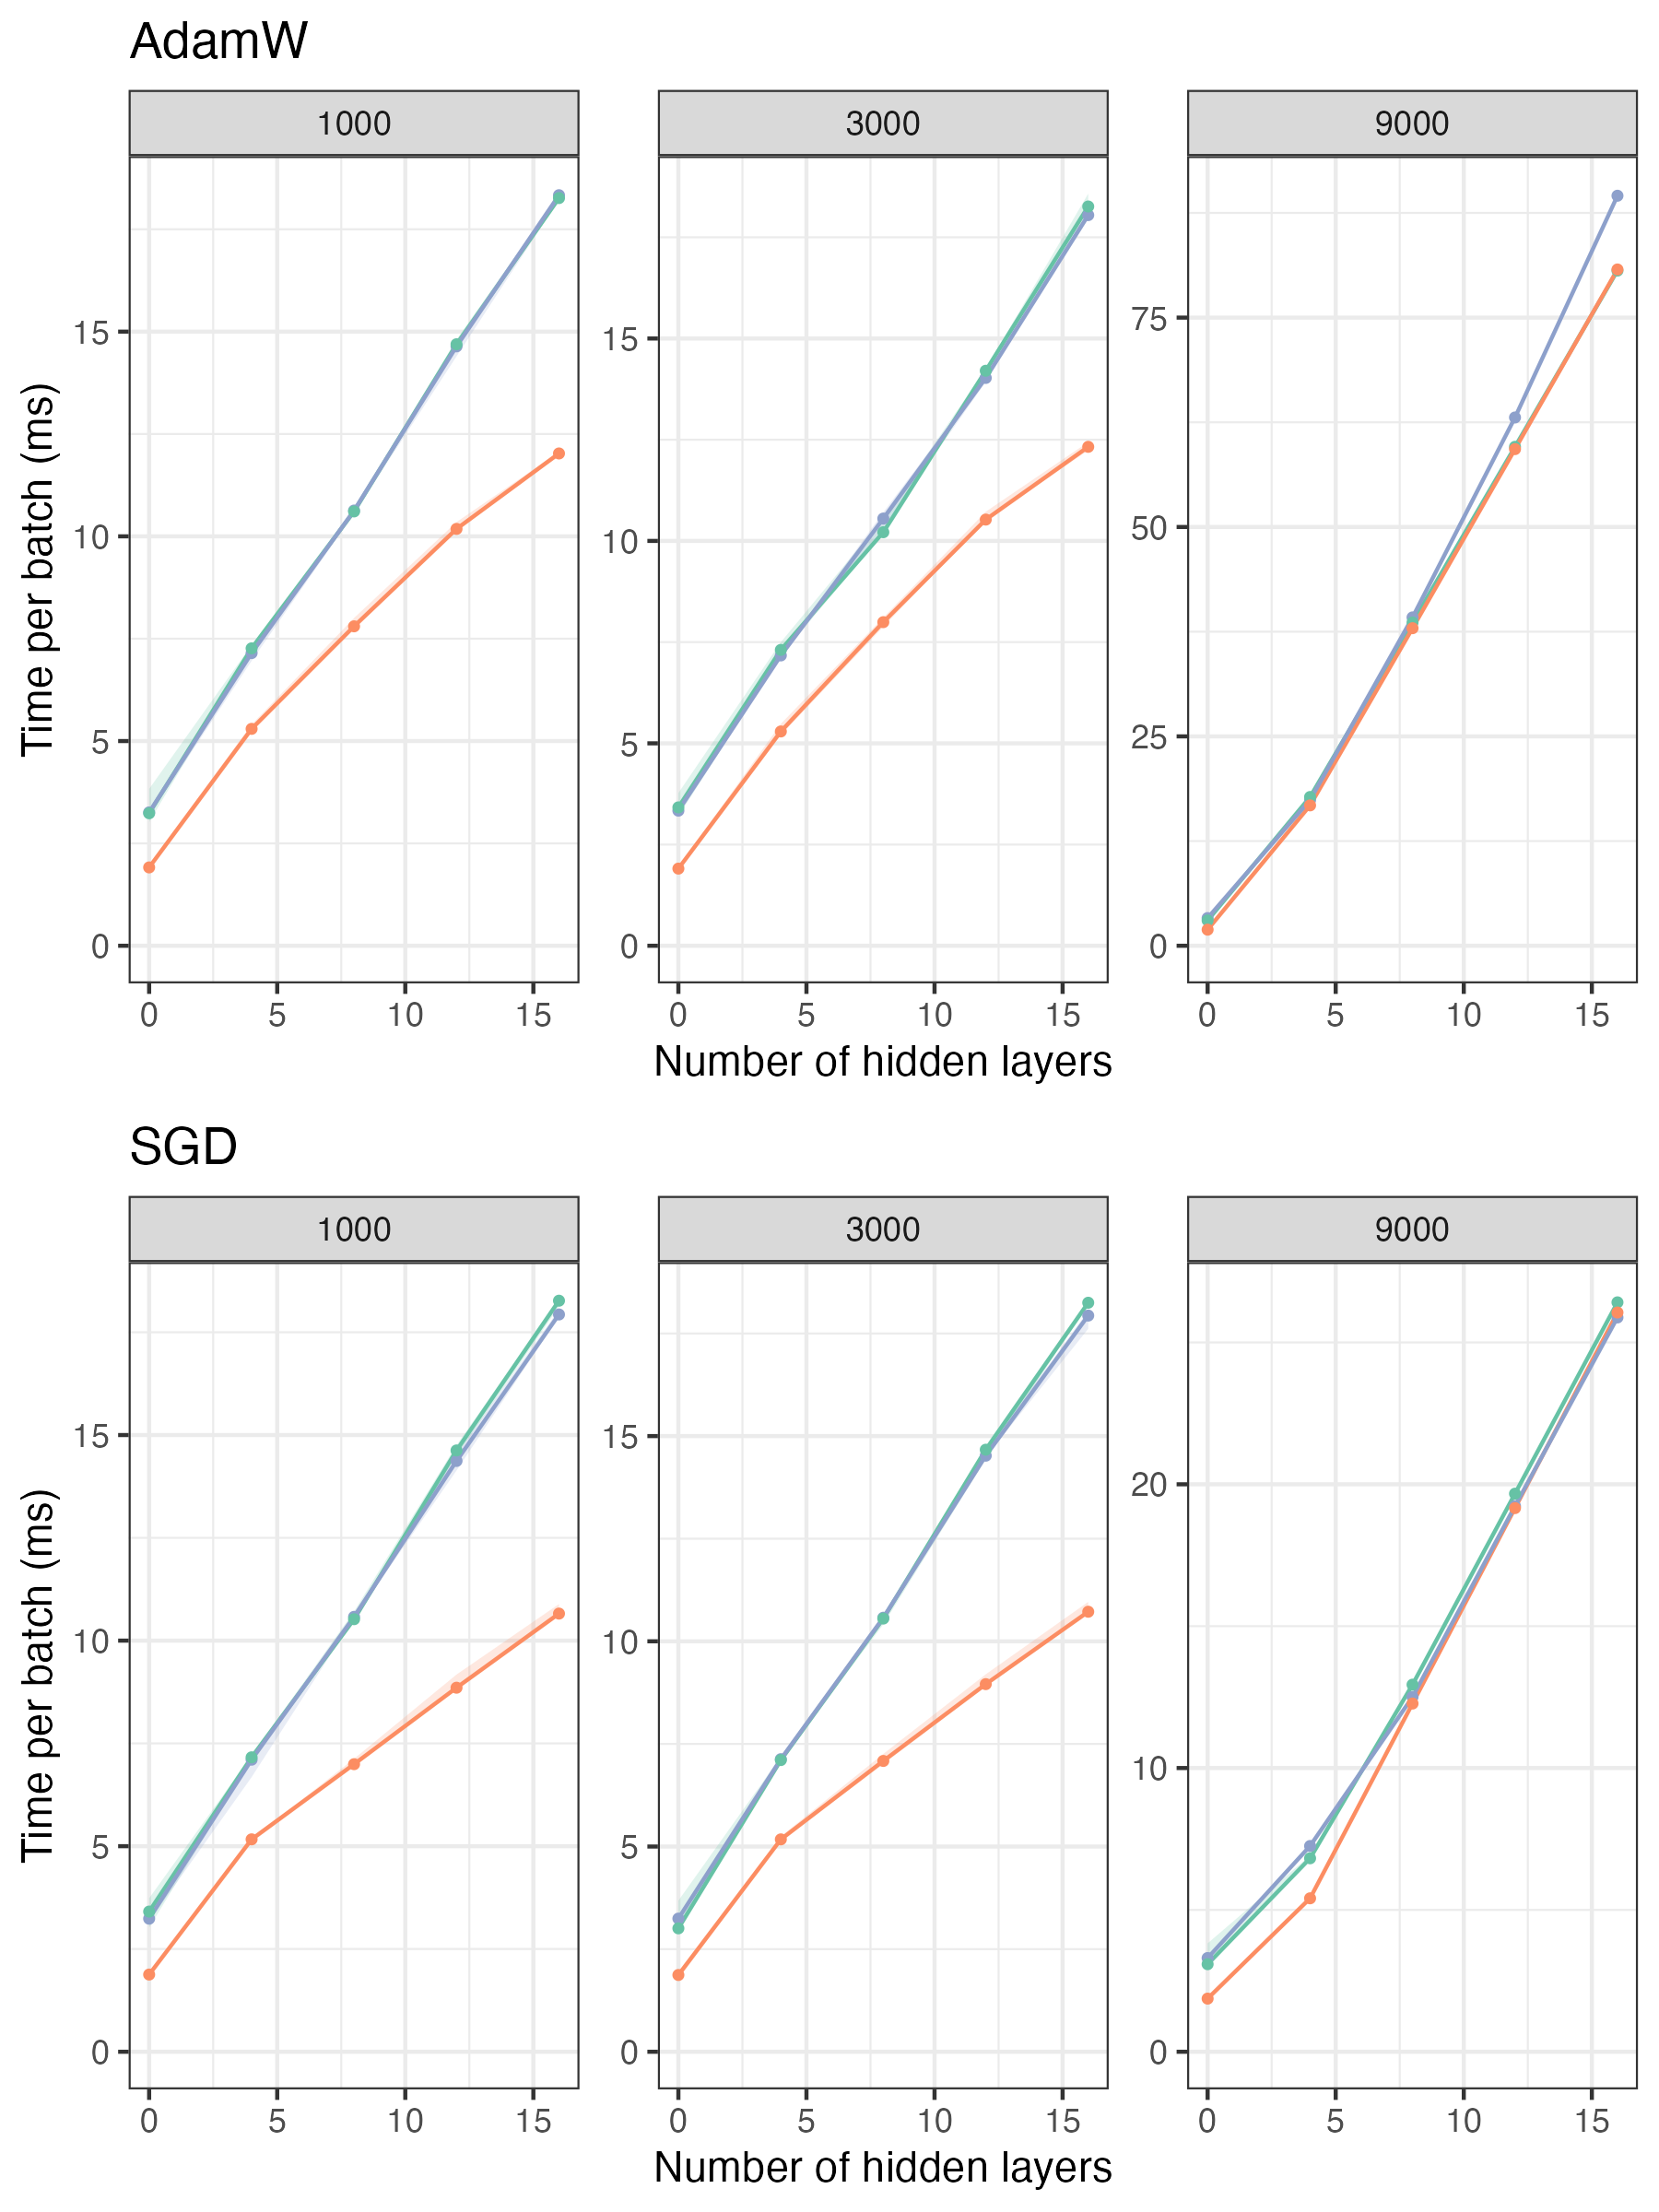
\includegraphics[width=0.8\textwidth]{figures/plot_adamw.png}
    \caption{Runtime results for the AdamW optimizer. The facets represent different latent dimensions.}
    \label{fig:adamw-benchmark}
\end{figure}

Next, \Cref{fig:sgd-benchmark} presents the same runtime benchmarks when using the SGD optimizer.
In this scenario, \pytorch{} achieves the best performance for all configurations.
Because the optimizer is considerably simpler, using the \libtorch{} implementation has less of an effect on the runtime.

\begin{figure}[h]
    \centering
    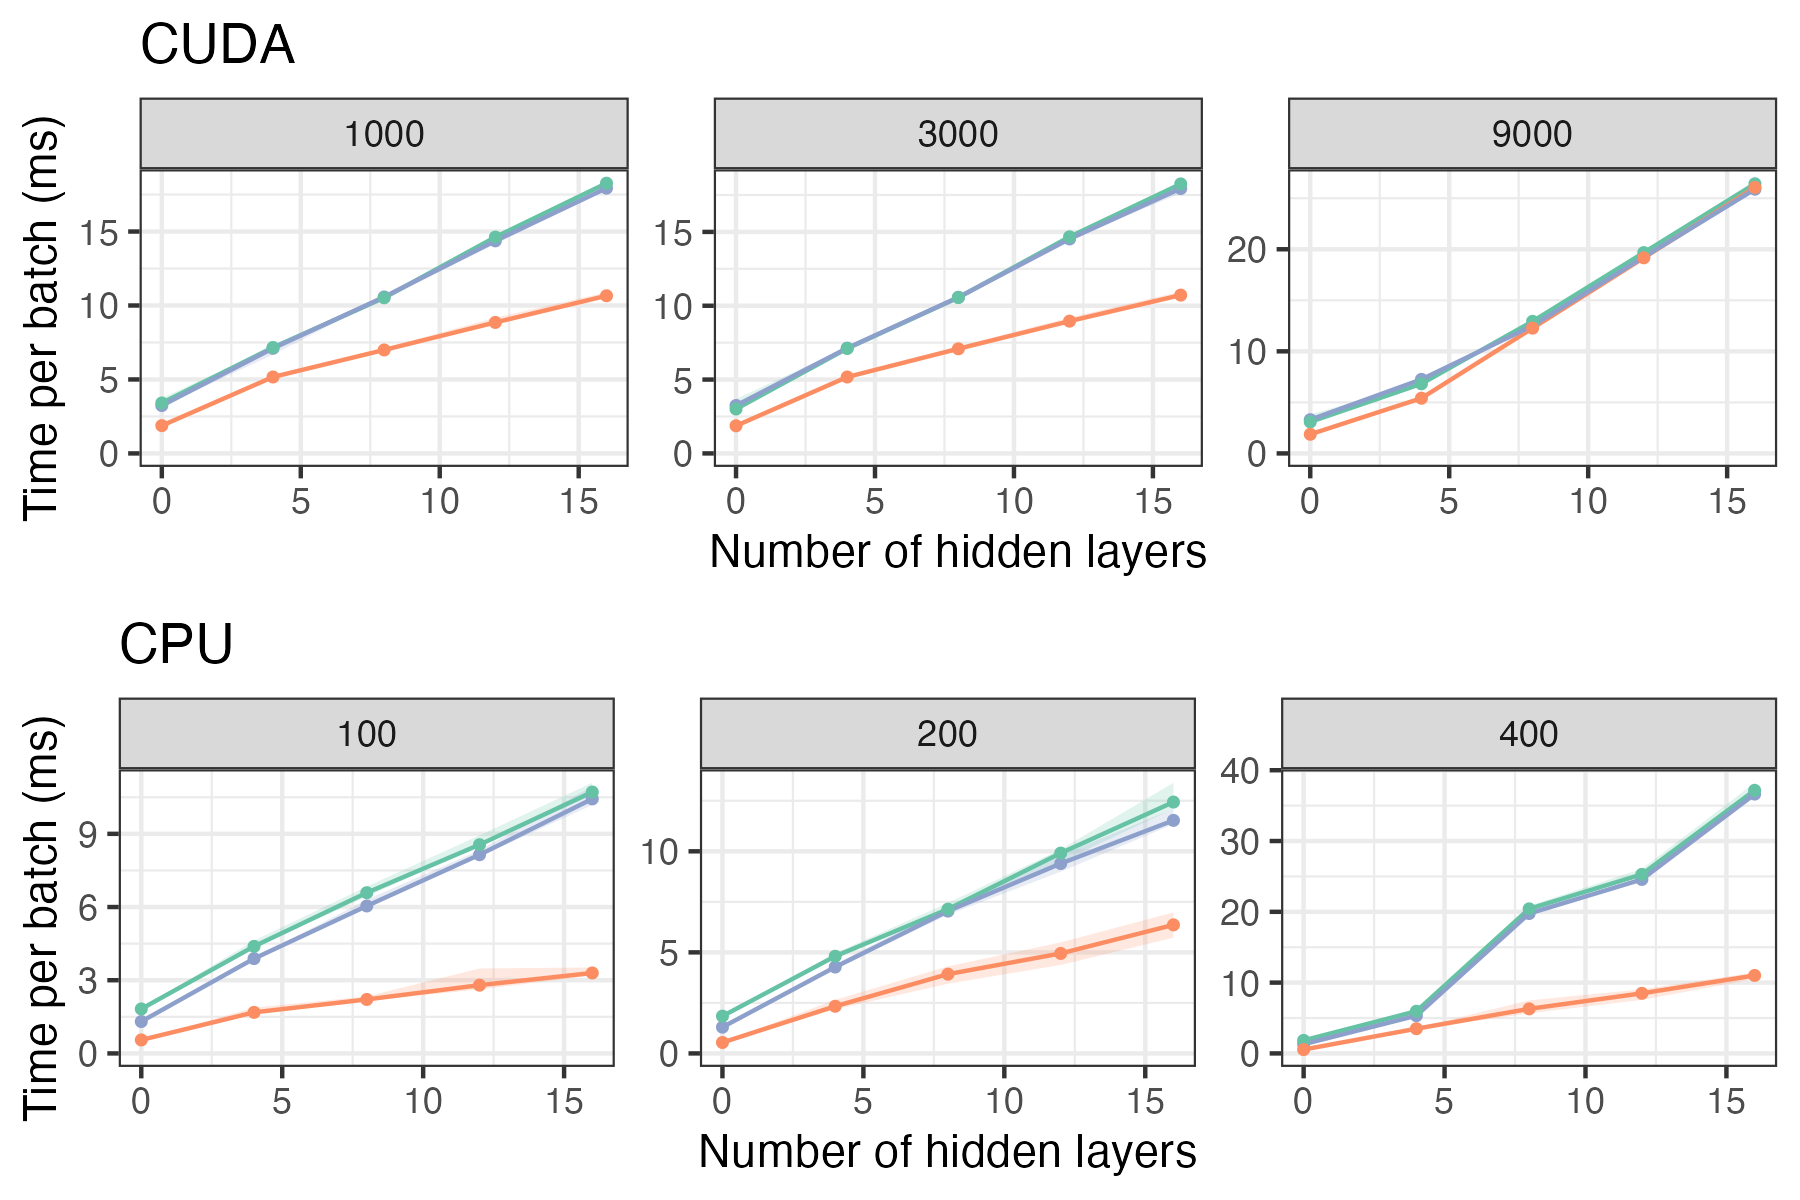
\includegraphics[width=0.8\textwidth]{figures/plot_sgd.png}
    \caption{Runtime results for the SGD optimizer. The facets represent different latent dimension.}
    \label{fig:sgd-benchmark}
\end{figure}

In summary, we recommend using the ignite versions of the optimizer to obtain good runtime performance and, if possible, jit-compiling the network (via \code{torch::jit\_trace} or the \code{jit\_trace} parameter in \mlrttorch{}).

\section{Conclusion}\label{sec:conclusion}

In this work, we introduced \pkg{mlr3torch}, which offers an extensive deep learning framework in \rlang{} that integrates with the \mlrt{} ecosystem.
This enables seamless access to operations like resampling, benchmarking, and hyperparameter tuning.

The package offers a unified interface for defining, training, and evaluating neural networks, with support for both tabular data and generic tensors in supervised classification and regression tasks.
Neural network architectures are available in different levels of control: Predefined architectures are readily available, \torch{} modules can be easily converted to \mlrttorch{} learners, and custom architectures can be defined as graphs.
Enabled by the lazy tensor type and the integration with \mlrtpipelines{}, the whole modeling workflow, including preprocessing, data augmentation, and the neural network itself, can be represented as a single graph.

A key strength of \pkg{mlr3torch} is its extensibility and flexibility, be it in defining architectures, customizing the training, e.g., via the provided callback mechanism, or extending the package to new task types.
We demonstrated the package's capabilities through three practical use cases: First, we showed how to perform neural architecture search on a tabular regression problem. Second, we fine-tuned a pre-trained ResNet-18 model to a binary image classification task.Finally, we showcased the framework's ability to define architectures with multiple inputs for a multi-modal task that contained both tabular data and images.

Our runtime benchmarks demonstrate that the framework overhead compared to pure \torch{} implementations is minimal, and that the right configuration yields good runtime performance compared to \pytorch{}.

Future development will focus on extending support to other learning tasks such as survival analysis, implementing additional architectures, further improving runtime performance, and extending the support to other modalities like natural language.

\section*{Acknowledgements}

Sebastian Fischer is supported by the Deutsche Forschungsgemeinschaft (DFG, German Research Foundation) – 460135501 (NFDI project MaRDI).

\bibliography{refs}

\begin{appendix}

\section{Computational details}\label{app:comp-details}

\begin{itemize}
    \item CUDA Version
    \item R version
    \item torch, mlr3torchm pytorch version
    \item GPU
    \item OS
    \item VRAM
\end{itemize}

\end{appendix}


\end{document}
